\documentclass[10pt]{scrartcl}

%Math
\usepackage{amsmath}
\usepackage{amsfonts}
\usepackage{amssymb}
\usepackage{amsthm}
\usepackage{ulem}
\usepackage{stmaryrd} %f\UTF{00FC}r Blitz!

%PageStyle
\usepackage[ngerman]{babel} % deutsche Silbentrennung
\usepackage[utf8]{inputenc} 
\usepackage{fancyhdr, graphicx}
\usepackage[scaled=0.92]{helvet}
\usepackage{enumitem}
\usepackage{parskip}
\usepackage[a4paper,top=2cm]{geometry}
\setlength{\textwidth}{17cm}
\setlength{\oddsidemargin}{-0.5cm}
\usepackage[scaled=0.92]{helvet}
\usepackage{lastpage} % for getting last page number
\renewcommand{\familydefault}{\sfdefault}


% Shortcommands
\newcommand{\Bold}[1]{\textbf{#1}} %Boldface
\newcommand{\Kursiv}[1]{\textit{#1}} %Italic
\newcommand{\T}[1]{\text{#1}} %Textmode
\newcommand{\Nicht}[1]{\T{\sout{$ #1 $}}} %Streicht Shit durch

%Arrows
\newcommand{\lra}{\leftrightarrow} 
\newcommand{\ra}{\rightarrow}
\newcommand{\la}{\leftarrow}
\newcommand{\lral}{\longleftrightarrow}
\newcommand{\ral}{\longrightarrow}
\newcommand{\lal}{\longleftarrow}
\newcommand{\Lra}{\Leftrightarrow}
\newcommand{\Ra}{\Rightarrow}
\newcommand{\La}{\Leftarrow}
\newcommand{\Lral}{\Longleftrightarrow}
\newcommand{\Ral}{\Longrightarrow}
\newcommand{\Lal}{\Longleftarrow}

% Code listenings
\usepackage{color}
\usepackage{xcolor}
\usepackage{listings}
\usepackage{caption}
\DeclareCaptionFont{white}{\color{white}}
\DeclareCaptionFormat{listing}{\colorbox{gray}{\parbox{\textwidth}{#1#2#3}}}
\captionsetup[lstlisting]{format=listing,labelfont=white,textfont=white}
\lstdefinestyle{JavaStyle}{
 language=Java,
 basicstyle=\footnotesize\ttfamily, % Standardschrift
 numbers=left,               % Ort der Zeilennummern
 numberstyle=\tiny,          % Stil der Zeilennummern
 stepnumber=5,              % Abstand zwischen den Zeilennummern
 numbersep=5pt,              % Abstand der Nummern zum Text
 tabsize=2,                  % Groesse von Tabs
 extendedchars=true,         %
 breaklines=true,            % Zeilen werden Umgebrochen
 frame=b,         
 %commentstyle=\itshape\color{LightLime}, Was isch das? O_o
 %keywordstyle=\bfseries\color{DarkPurple}, und das O_o
 basicstyle=\footnotesize\ttfamily,
 stringstyle=\color[RGB]{42,0,255}\ttfamily, % Farbe der String
 keywordstyle=\color[RGB]{127,0,85}\ttfamily, % Farbe der Keywords
 commentstyle=\color[RGB]{63,127,95}\ttfamily, % Farbe des Kommentars
 showspaces=false,           % Leerzeichen anzeigen ?
 showtabs=false,             % Tabs anzeigen ?
 xleftmargin=17pt,
 framexleftmargin=17pt,
 framexrightmargin=5pt,
 framexbottommargin=4pt,
 showstringspaces=false      % Leerzeichen in Strings anzeigen ?        
}

 
\fancypagestyle{firststyle}{ %Style of the first page
\fancyhf{}
\fancyheadoffset[L]{0.6cm}
\lhead{

\includegraphics[scale=0.8]{./fhnw_ht_e_10mm.jpg}}
\renewcommand{\headrulewidth}{0pt}
\lfoot{Institute of computer science,\linebreak www.fhnw.ch }
}

\fancypagestyle{documentstyle}{ %Style of the rest of the document
\fancyhf{}
\fancyheadoffset[L]{0.6cm}
\lhead{

\includegraphics[scale=0.8]{./fhnw_ht_e_10mm.jpg}}
\renewcommand{\headrulewidth}{0pt}
\lfoot{\thepage\ / \pageref{LastPage} }
}

\pagestyle{firststyle} %different look of first page
 
\title{ %Titel
EAF Zusammenfassung}
\author{Jonas Schwammberger, Fabio Oesch \& Jan Fässler}

 \begin{document}
 \maketitle
 \thispagestyle{firststyle}
 \pagestyle{firststyle}
 

 \pagestyle{documentstyle}
 \tableofcontents
 \pagebreak
\section{Spring Framework}
\begin{center}
	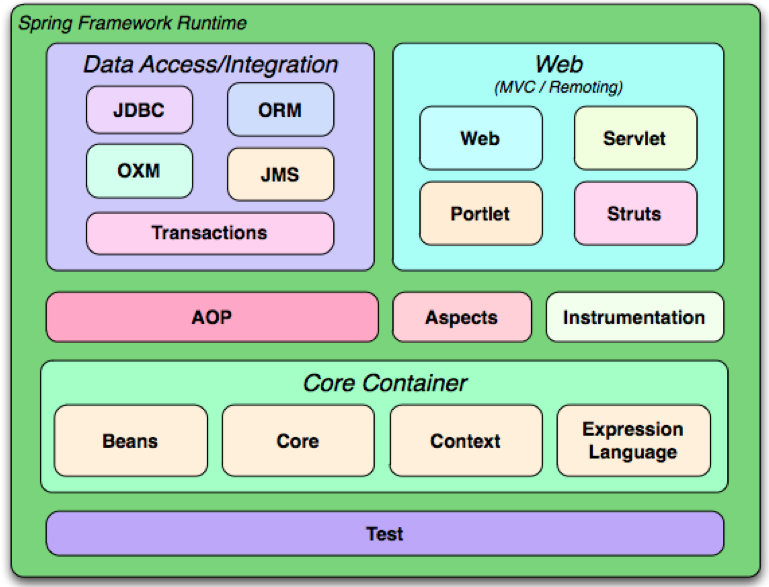
\includegraphics[scale=0.3]{spring.png}
\end{center}
\subsection{Grundsätze}
\begin{description}
	\item[Dependency Injection] \hfill \\
		Den Objekten werden die benötigten Ressourcen und Objekte zugewiesen. Sie müssen sie nicht selbst suchen.
	\item[Aspekt-orientierte Programmierung] \hfill \\
		Dadurch kann man vor allem technische Aspekte wie Transaktionen oder Sicherheit isolieren und den eigentlichen Code davon frei halten.
	\item[Templates] \hfill \\
		Vorlagen dienen dazu, die Arbeit mit einigen Programmierschnittstellen (APIs) zu vereinfachen, indem Ressourcen automatisch aufgeräumt sowie Fehlersituationen einheitlich behandelt werden.
\end{description}
\subsubsection{Dependency Injection}
Dieses Paradigma beschreibt die Arbeitsweise von Frameworks: eine Funktion eines Anwendungsprogramms wird bei einer Standardbibliothek registriert und von dieser zu einem späteren Zeitpunkt aufgerufen. Statt dass die Anwendung den Kontrollfluss steuert und lediglich Standardfunktionen benutzt, wird die Steuerung der Ausführung bestimmter Unterprogramme an das Framework abgegeben.
\subsubsection{Aspect-oriented}
AOP ist ein Programmierparadigma, um verschiedene logische Aspekte einer Anwendung getrennt voneinander zu entwerfen, zu entwickeln und zu testen. Die getrennt entwickelten Aspekte werden dann zur endgültigen Anwendung zusammengefügt. In Enterprise Applikationen werden mit AOP vor allem System Services, wie Transaktion, Sicherheit, ... von der Business Logik entkoppelt, so dass sich der Programmierer beim Erstellen des Business Objekte vollkommen auf die Geschäftslogik und dadurch auf den eigentlichen Verwendungszweck der Applikation konzentrieren kann.
\subsubsection{Container}
Spring ist ein Container, d.h. er enthält und verwaltet den Lebenszyklus und die Konfiguration von Java-Objekten. Die Java-Objekte sind sogenannte POJOs (Plain-Old-Java- Objects). Der Spring Container kann schnell herunter- und hinaufgefahren werden. Das ermöglicht eine effiziente Entwicklung und einen gezielten Einsatz für Unit. Tests. Der Spring Container kann beispielsweise explizit für einen Unit-Test hochgefahren werden. Der Container kann problemlos im Java EE, Java SE und in Webapplikationen integriert werden. Auch setzt er keine spezielle Architektur voraus und benötigt keine umgebungsspezifischen Konfigurationsdateien. Spring wird einfach mit einer entsprechenden Applikation mitgeliefert.
\subsection{Configuration}
\begin{center}
	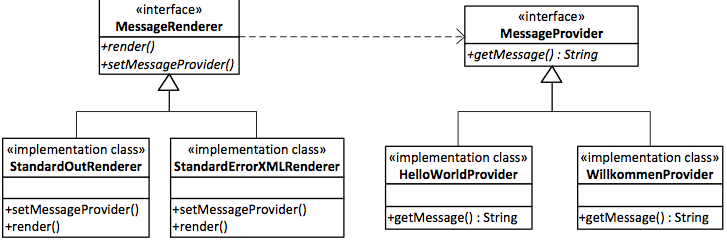
\includegraphics[scale=0.4]{simpleSpringApp.png}
\end{center}
\subsubsection{XML Based}
Vor/Nachteile:
\begin{itemize}
	\item[+] Keine Kompilation nach Konfigurationsänderung
	\item[+] XML ist bekannt
	\item[+] Tool unterstützung vorhanden
	\item[+] Zentrales XML-File, dadurch abhängigkeiten gut ersichtlich
	\item[-] Kann bei grossen Projekten unübersichtlich werden
	\item[-] Implementation und Konfiguration sind von einander getrennt
\end{itemize}
\lstinputlisting[caption=SimpleSpringApp,style=JavaStyle]{simpleSpringApp.java}
\lstinputlisting[caption=helloConfig.xml,style=JavaStyle]{simpleSpringApp.xml}
\subsubsection{Annotation Based}
Vor/Nachteile:
\begin{itemize}
	\item[+] Implementation und Konfiguration sind zusammen
	\item[+] keine riesen XML
	\item[-] Bei grossen Projekten ist es schwierig den Überblick zu behalten
	\item[-] Der Java Quellcode muss zur Verfügung stehen
\end{itemize}
\lstinputlisting[caption=Annotation based,style=JavaStyle]{annotationSpringApp.java}
\lstinputlisting[caption=helloConfig.xml,style=JavaStyle]{annotationSpringApp.xml}
\subsubsection{Java Based}
\begin{itemize}
	\item[+] Implementation und Konfiguration sind zusammen
	\item[+] Alles in Java, kein XML
	\item[+] Gute Tool Unterstützung
	\item[-] Konfigurationsänderungen führen zur Komplilation der Konfigurationsklasse
\end{itemize}
\lstinputlisting[caption=JavaConfig,style=JavaStyle]{javaSpringApp.java}

\newpage
\section{Java Persistence API (JPA)}
\subsection{General Info}
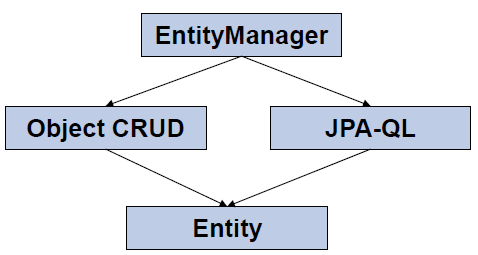
\includegraphics[scale=0.5]{jpa.png}\\
\Bold{JPA Components}
\begin{itemize}
\item EntityManager provides access to the objects (similar to a DAO)\\
$\bullet$ find / persist / update / remove\\
$\bullet$ Query API and JPA-QL
\item Controlled Lifecycle
\end{itemize}
\Bold{Entity Metadata}
\begin{itemize}
\item Form:\\
$\bullet$ Annotations\\
$\bullet$ XML Files
\item Configuration by Exception
\end{itemize}
\subsection{Entity Annotations}
\lstinputlisting[label=Entity,caption=Entity]{entity.java}
Folie 10 - 19, Foliensatz JPA1.pdf sind Spezifikationen und Anforderungen an Entity Klasse
\subsubsection{Primary Keys: Generation}
\begin{itemize}
\item Assigned\\
$\bullet$ Primary keys may be assigned by application, i.e. no key generation\\
\hspace*{0.5cm}$\bullet$ E.g. language table: Primary Key is the ISO country code
\item Identity\\
$\bullet$ Auto increment supported by some DBs
\item Sequence\\
$\bullet$ Some DBs support sequences which generate unique values (e.g. Oracle, PostgreSql)
\item Table\\
$\bullet$ Primary keys are stored in a separate PK table
\end{itemize}
\Bold{Performance Comparison}
\begin{itemize}
\item 10'000 insert statements
\item AUTO (Identity) 7534 msec
\item TABLE (allocationSize = 32768) 2244 msec
\item TABLE (allocationSize = 1) 9612 msec
\item TABLE (allocationSize = 2) 7429 msec
\item TABLE (allocationSize = 4) 5856 msec
\item ASSIGNED (user defined) 1959 msec
\end{itemize}
\subsubsection{Associations}
\begin{itemize}
\item OneToOne, owning side contains the foreign key
\item OneToMany
\item ManyToOne
\item ManyToMany, either side may be the owning side
\item Owning side determines the updates to the relationships in the database
\end{itemize}
\Bold{Relationships can be:}
\begin{itemize}
\item Unidirectional\\
$\bullet$ Has an owning side
\item Bidirectional\\
$\bullet$ Has an owning side\\
$\bullet$ Has an inverse side
\end{itemize}
\Bold{ManyToOne: User - Rental: bidirectional}\\
Bei bidirektionalen Beziehungen sind die Many-Side die owning Side. \\
Example:
\lstinputlisting[label=Example,caption=Example]{example.java}
Inverse Side Example:
\lstinputlisting[label=InverseSideExample,caption=InverseSideExample]{inverseSideExample.java}
\Bold{Only references from $n$ to $1$ are persisted!}
\lstinputlisting[label=OneToMany bidirectional,caption=OneToMany bidirectional]{OneToMany.java}
\begin{itemize}
\item the two orders are stored in the DB (due to the cascade=PERSIST)
\item the associations are NOT persisted!!!
\end{itemize}
\subsubsection*{OneToOne / OneToMany / ManyToOne / ManyToMany - Attributes}
\begin{itemize}
\item fetch EAGER / LAZY\\
$\bullet$ determines fetch type
\item cascade MERGE / PERSIST / REFRESH / DETACH REMOVE / ALL\\
$\bullet$ determines cascade operation
\item mappedBy String, not for ManyToOne\\
$\bullet$ used for bidirectional associations (on the inverse side)
\item optional boolean, only for OneToOne/ManyToOne\\
$\bullet$ determines, whether null is possible (0..1)
\item orphanRemoval boolean, only for OneToOne/OneToMany
\end{itemize}
\Bold{Example:}\\
@OneToOne(cascade={CascadeType.PERSIST, CascadeType.REMOVE})\\
Slides 20 \& 21, Foliensatz JPA2\_ Slides.pdf Cascading und Fetch Types werden erklärt\\
Im Zusammenhang mit Fetch Types ist Lazy Loading Problem erklärt im Foliensatz 00\_ JPA2\_ Arbeitsblatt\_ Besprechung.pdf
\Bold{Inheritance}\\
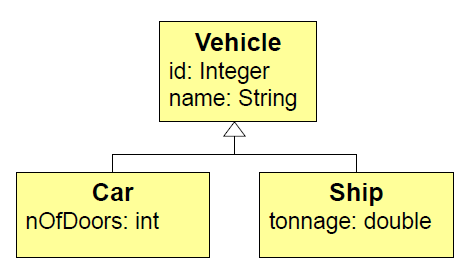
\includegraphics[scale=0.5]{inheritance.png}
\subsubsection{Examples}
\lstinputlisting[label=Example,caption=Example]{Example2.java}
\begin{itemize}
\item Representation\\
$\bullet$ SINGLE TABLE (default)\\
$\bullet$ TABLE\_ PER\_ CLASS (per concrete class a table is defined)\\
$\bullet$ JOINED (one table per class)
\item Specification\\
$\bullet$ Inheritance type can be specified on root entity using @Inheritance annotation
\end{itemize}
\Bold{Single Table Example (@Inheritance(strategy=InheritanceType.SINGLE\_TABLE))}\\
\begin{tabular}{|l|l|l|l|l|}
\hline
DTYPE&ID&NAME&NOFDOORS&TONNAGE\\\hline
Car&1&VW Sharan&5&(null)\\\hline
Car&2&Smart&2&(null)\\\hline
Ship&3&Queen Mary&(null)&76000\\\hline
\end{tabular}
\Bold{Disadvantages}\\
$\bullet$ All fields added in subclasses must be nullable\\
$\bullet$ Foreign keys can only refer to the base class\\
\Bold{Joined Table Example (@Inheritance(strategy=InheritanceType.JOINED))}\\
\begin{tabular}{|l|l|}
\hline
ID&NAME\\\hline
1&VW Sharan\\\hline
2&Smart\\\hline
3&Queen Mary\\\hline
\end{tabular}
\hspace*{1cm}
\begin{tabular}{|l|l|}
\hline
ID&NOFDOORS\\\hline
1&5\\\hline
2&2\\\hline
\end{tabular}
\hspace*{1cm}
\begin{tabular}{|l|l|}
\hline
ID&TONNAGE\\\hline
3&76000\\\hline
\end{tabular}
\begin{itemize}
\item Advantages:\\
$\bullet$normalized schema, a database table for each class\\
$\bullet$ All fields can be defined with not null conditions\\
$\bullet$ Foreign-key references to concrete subclasses are possible
\item Disadvantages:\\
$\bullet$ Each entity access has to go over several tables
\end{itemize}
\Bold{TABLE\_ PER\_ CLASS Table Example (@Inheritance(strategy=InheritanceType.TABLE\_ PER\_ CLASS))}\\
\begin{tabular}{|l|l|l|}
\hline
ID&NAME&NOFDOORS\\\hline
1&VW Sharan&5\\\hline
2&Smart&2\\\hline
\end{tabular}
\hspace*{1cm}
\begin{tabular}{|l|l|l|}
\hline
ID&NAME&TONNAGE\\\hline
3&Queen Mary&76000\\\hline
\end{tabular}
\begin{itemize}
\item Advantages:\\
$\bullet$ Non-null constraints can be defined\\
$\bullet$ Foreign-key references to concrete subclasses are possible (but not to abstract base classes)
\item Disadvantages:\\
$\bullet$ Polymorphic queries need to access several tables\\
$\bullet$ Identity generator cannot be used\\
$\bullet$ Not required by JPA 2.0-Spec (but provided by Hibernate)
\end{itemize}
\subsection{Entity Manager}
Entity Manager API auf Seite 8-11, Foliensatz JPA2\_ Slides.pdf\\
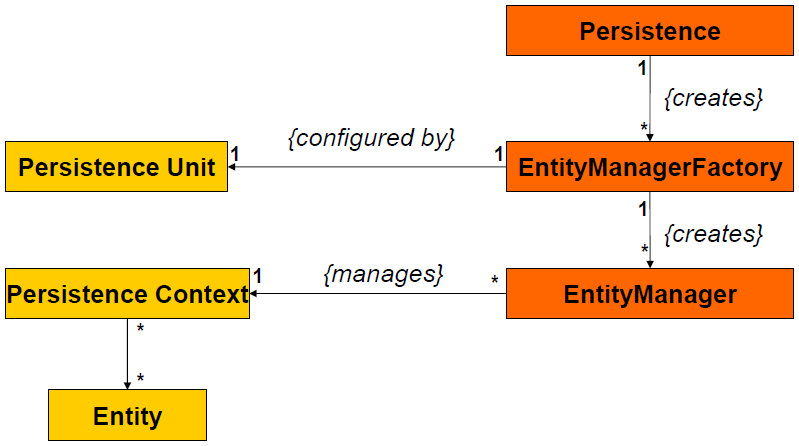
\includegraphics[scale=0.5]{entitymanager.png}\\
\Bold{Only one Java instance with the same persistent identity may exist in a Persistence Context}\\
\lstinputlisting[label=Access to Entity Manager,caption=Access to Entity Manager]{accessEntityManager.java}
\subsubsection{Queries}
\begin{itemize}
\item JPQL\\
$\bullet$ Used to query/manipulate database\\
$\bullet$ Inspired by SQL, but it operates directly on the entities and its fields
\item Statements\\
$\bullet$ select\_ statement ::= select\_ clause from\_ clause [where\_ clause] [groupby\_ clause] [having\_ clause] [orderby\_ clause]\\
$\bullet$ update\_ statement ::= update\_ clause [where\_ clause]\\
$\bullet$ delete\_ statement ::= delete\_ clause [where\_ clause]
\end{itemize}
\subsection{Transactions}
\Bold{Access to the EntityManager must run within a transaction}
\subsection{Data Transfer Object}
\begin{itemize}
\item Detached Entity objects as DTOs\\
$\bullet$ Hibernate developers say that you can use hibernate entity or domain objects as result types in service methods\\
$\bullet$ Problems:\\
\hspace*{0.5cm}$\bullet$ Lazy load exceptions are thrown if "not-loaded" fields are accessed\\
\hspace*{0.5cm}$\bullet$Having an accessor which does throw an exception is contract violating\\
\hspace*{0.5cm}$\bullet$Accessing the type of a result using reflection returns a proxy type (which is not serializable)
\item Data Transfer Objects\\
$\bullet$ Are used to transfer data across layers of your application\\
$\bullet$ Only the data needed by the requesting layer are passed, i.e. not all properties need to be\\
$\bullet$ No Lazy Loading Exception surprises\\
$\bullet$ Clients are independent of ORM technology used
\end{itemize}
\subsubsection{Service Method (Dozer)}
\begin{itemize}
\item Dozer is a Java Bean to Java Bean mapper that recursively copies data from one object to another $\Ra$ can be used to copy DTO
\item Dozer supports simple property mapping, complex type mapping, bi-directional mapping, implicit-explicit mapping, as well as recursive mapping. This includes mapping collection attributes that also need mapping at the element level
\end{itemize}
\subsubsection{Con}
\begin{itemize}
\item Code Duplication\\
$\bullet$ In particular when DTOs have the same fields as domain objects
\item Code to copy attributes back and forth\\
$\bullet$ Dozer / Spring BeanUtils / JPA
\end{itemize}
\subsubsection{Pro}
\begin{itemize}
\item Lazy Loading Problem\\
$\bullet$ You are not catched by a Lazy Loading Exception\\
\hspace*{0.5cm}$\bullet$ neither on client side\\
\hspace*{0.5cm}$\bullet$nor upon serialization
\item Triggers Design\\
$\bullet$ Forces you to think about the interface of the remote service façades\\
$\bullet$ Information from multiple domain objects can be combined in one DTO
\end{itemize}

\newpage
\section{Spring Remoting}
\subsection{Prüfung}
\begin{description}
\item[Facade:] Zuständig für abstraktion von Service Layer und benutzt am besten DTO's
\item[Service Layer:] Service Schnittstellen stellt Business Cases dar
\item[Domain Model:] Entities
\item[Database Access:] Wird von JPA Implementation übernommen
\end{description}
\section{Anhang}
\lstinputlisting[label=Persistence Unit,caption=Persistence Unit]{persistance.java}
\lstinputlisting[label=Query Examples,caption=Query Examples]{queries.java}

\end{document}